\documentclass{article} % For LaTeX2e
\usepackage{iclr2018_conference,times}
 % \usepackage{hyperref}
\usepackage{url}

\usepackage[T1]{fontenc}  
\usepackage[utf8]{inputenc}             
 % \usepackage[english,french]{babel}  
\usepackage[english]{babel} 

\usepackage{graphicx}
\usepackage{caption}
\usepackage{booktabs}
\usepackage{enumitem}

\usepackage{amsmath}
\usepackage{amsfonts}
\usepackage{amsthm}

\newcommand*\samethanks[1][\value{footnote}]{\footnotemark[#1]}

\title{Breaking the Softmax Bottleneck: \\ A High-Rank RNN Language Model}

% Authors must not appear in the submitted version. They should be hidden
% as long as the \iclrfinalcopy macro remains commented out below.
% Non-anonymous submissions will be rejected without review.

\author{Zhilin Yang\thanks{Equal contribution. Ordering determined by dice rolling.}~~, Zihang Dai\samethanks~~, Ruslan Salakhutdinov, William W. Cohen\\
School of Computer Science\\
Carnegie Mellon University\\
\texttt{\{zhiliny,dzihang,rsalakhu,wcohen\}@cs.cmu.edu}
}

% The \author macro works with any number of authors. There are two commands
% used to separate the names and addresses of multiple authors: \And and \AND.
%
% Using \And between authors leaves it to \LaTeX{} to determine where to break
% the lines. Using \AND forces a linebreak at that point. So, if \LaTeX{}
% puts 3 of 4 authors names on the first line, and the last on the second
% line, try using \AND instead of \And before the third author name.

% table cell
\usepackage{array}
\newcolumntype{C}{>{\centering\arraybackslash}p{0.15\linewidth}}

% table cell length
\newlength\contextlength 
\setlength\contextlength{\linewidth}

% special token
\newcommand{\blank}{\_\_?\_\_}

\newcommand{\fix}{\marginpar{FIX}}
\newcommand{\new}{\marginpar{NEW}}
\newcommand{\todo}[1]{{\color{red} TODO: {#1}}}

\iclrfinalcopy % Uncomment for camera-ready version, but NOT for submission.

\newtheorem{lemma}{Lemma}
\newtheorem{prop}{Proposition}
\newtheorem{coro}{Corollary}
\newtheorem{property}{Property}

\begin{document}


\maketitle

\begin{abstract}
We formulate language modeling as a matrix factorization problem, and show that the expressiveness of Softmax-based models (including the majority of neural language models) is limited by a {\em Softmax bottleneck}. Given that natural language is highly context-dependent, this further implies that in practice Softmax with distributed word embeddings does not have enough capacity to model natural language. We propose a simple and effective method to address this issue, and improve the state-of-the-art perplexities on Penn Treebank and WikiText-2 to 47.69 and 40.68 respectively. The proposed method also excels on the large-scale 1B Word dataset, outperforming the baseline by over 5.6 points in perplexity.\footnote{Code is available at \url{https://github.com/zihangdai/mos}.}
\end{abstract}

\section{Introduction}
\label{sec:intro}

Language modeling is among the important problems that require modeling long-term dependency, with successful applications such as unsupervised pretraining~\citep{dai2015semi,peters2018deep,radford2018improving,devlin2018bert}.
However, it has been a challenge to equip neural networks with the capability to model long-term dependency in sequential data.
Recurrent neural networks (RNNs), in particular Long Short-Term Memory (LSTM) networks~\citep{hochreiter1997long}, have been a standard solution to language modeling and obtained strong results on multiple benchmarks.
Despite the wide adaption, RNNs are difficult to optimize due to gradient vanishing and explosion~\citep{hochreiter2001gradient}, and the introduction of gating in LSTMs and the gradient clipping technique~\citep{graves2013generating} might not be sufficient to fully address this issue.
% ,pascanu2012understanding
Empirically, previous work has found that LSTM language models use 200 context words on average~\citep{khandelwal2018sharp}, indicating room for further improvement.

On the other hand, the direct connections between long-distance word pairs baked in attention mechanisms might ease optimization and enable the learning of long-term dependency~\citep{bahdanau2014neural,vaswani2017attention}.
Recently, \citet{al2018character} designed a set of auxiliary losses to train deep Transformer networks for character-level language modeling, which outperform LSTMs by a large margin.
Despite the success, the LM training in~\citet{al2018character} is performed on separated fixed-length segments of a few hundred characters, without any information flow across segments.
As a consequence of the fixed context length, the model cannot capture any longer-term dependency beyond the predefined context length.
In addition, the fixed-length segments are created by selecting a consecutive chunk of symbols without respecting the sentence or any other semantic boundary.
Hence, the model lacks necessary contextual information needed to well predict the first few symbols, leading to inefficient optimization and inferior performance.
We refer to this problem as \textit{context fragmentation}.

%However, the context length is fixed to hundreds of characters and thus it is not possible to model longer-term dependency. Moreover, it is not clear how the model performs on word-level language modeling data, as the granularity changes.

% Moreover, using auxiliary losses brings additional challenges such as properly tuning the mixture weights and the loss decay schedule.

To address the aforementioned limitations of fixed-length contexts, we propose a new architecture called Transformer-XL (meaning extra long).
We introduce the notion of recurrence into our deep self-attention network. In particular, instead of computing the hidden states from scratch for each new segment, we reuse the hidden states obtained in previous segments.
The reused hidden states serve as memory for the current segment, which builds up a recurrent connection between the segments.
As a result, modeling very long-term dependency becomes possible because information can be propagated through the recurrent connections.
Meanwhile, passing information from the previous segment can also resolve the problem of context fragmentation.
More importantly, we show the necessity of using relative positional encodings rather than absolute ones, in order to enable state reuse without causing temporal confusion.
Hence, as an additional technical contribution, we introduce a simple but more effective relative positional encoding formulation that generalizes to attention lengths longer than the one observed during training.

Transformer-XL obtained strong results on five datasets, varying from word-level to character-level language modeling.
Transformer-XL is also able to generate relatively coherent long text articles with \textit{thousands of} tokens (see Appendix \ref{sec:gen}), trained on only 100M tokens.
% Transformer-XL improves the previous state-of-the-art (SoTA) results from 1.06 to 0.99 in bpc on enwiki8, from 1.13 to 1.08 in bpc on text8, from 20.5 to 18.3 in perplexity on WikiText-103, and from 23.7 to 21.8 in perplexity on One Billion Word.
% Transformer-XL improves the previous state-of-the-art (SoTA) results to 0.99 in bpc on enwiki8, 1.08 in bpc on text8, 18.3 in perplexity on WikiText-103, and 21.8 in perplexity on One Billion Word.
% On small data, Transformer-XL also achieves a perplexity of 54.5 on Penn Treebank without finetuning, which is SoTA when comparable settings are considered.

Our main technical contributions include introducing the notion of recurrence in a purely self-attentive model and deriving a novel positional encoding scheme. These two techniques form a complete set of solutions, as any one of them alone does not address the issue of fixed-length contexts. Transformer-XL is the first self-attention model that achieves substantially better results than RNNs on both character-level and word-level language modeling.

% On WikiText-103, Transformer-XL improves the previous state-of-the-art (SoTA) results from 33 perplexity to 24, with a relative reduction of 27\%. On enwiki8 character-level language modeling, Transformer-XL achieves a SoTA bpc of 1.03, which outperforms \cite{al2018character} by 0.03 with 60+\% fewer parameters. Given a more common model size with 40+M parameters, Transformer-XL achieves a bpc of 1.06, compared to 1.11 by \cite{al2018character}. Transformer-XL also achieves perplexities of 54.5 on Penn Treebank and 29.4 on One Billion Word, which are SoTA when comparable settings are considered.

% Due to the ability of modeling long-range context, our best model uses attention lengths of 1,600 and 3,800 on WikiText-103 and enwiki8 respectively. We also devise a metric called \textit{Relative Effective Context Length} (RECL) that aims to fairly compare the ability of long-range dependency modeling.
% % perform a fair comparison of the gains brought by increasing the context lengths for different models.
% In this setting, Transformer-XL learns a RECL of 900 words on WikiText-103, while the numbers for recurrent networks and Transformer are only 500 and 128.

% We use two methods to quantitatively study the effective lengths of Transformer-XL and the baselines. Similar to \cite{khandelwal2018sharp}, we gradually increase the attention length at test time until no further noticeable improvement ($\sim$0.1\% relative gains) can be observed. Our best model in this settings use attention lengths of 1,600 and 3,800 on WikiText-103 and enwiki8 respectively.
% %In addition, since the effective context length of Transformer-XL can be longer than the attention length due to our recurrent formulation, we devise a metric called \textit{Relative Effective Context Length} (RECL) that aims to perform a fair comparison of the gains brought by increasing the context lengths for different models.
% In addition, we devise a metric called \textit{Relative Effective Context Length} (RECL) that aims to perform a fair comparison of the gains brought by increasing the context lengths for different models.
% In this setting, Transformer-XL learns a RECL of 900 words on WikiText-103, while the numbers for recurrent networks and Transformer are only 500 and 128.


\section{Language Modeling as Matrix Factorization}\label{sec:rank}

As discussed in Section \ref{sec:intro}, with the autoregressive factorization, language modeling can be reduced to modeling the conditional distribution of the next token $x$ given the context $c$. Though one might argue that a natural language allows an infinite number of contexts due to its compositionality \citep{pinker1994language}, we proceed with our analysis by considering a finite set of possible contexts. The unboundedness of natural language does not affect our conclusions, which will be discussed later.

We consider a natural language as a finite set of pairs of a context and its conditional next-token distribution\footnote{We use capital letters for variables and small letters for constants.} $\mathcal{L} = \{(c_1, P^*(X | c_1)), \cdots, (c_N, P^*(X | c_N))\}$, where $N$ is the number of possible contexts. We assume $P^* > 0$ everywhere to account for errors and flexibility in natural language. Let $\{x_1, x_2, \cdots, x_M\}$ denote a set of $M$ possible tokens in the language $\mathcal{L}$. The objective of a language model is to learn a model distribution $P_\theta(X | C)$ parameterized by $\theta$ to match the true data distribution $P^*(X | C)$.

In this work, we study the expressiveness of the parametric model class $P_\theta(X | C)$.
In other words, we are asking the following question: given a natural language $\mathcal{L}$, does there exist a parameter $\theta$ such that $P_\theta(X | c) = P^*(X | c)$ for all $c$ in $\mathcal{L}$?

We start by looking at a Softmax-based model class since it is widely used.

\subsection{Softmax}

The majority of parametric language models use a Softmax function operating on a context vector (or hidden state) $\mathbf{h}_c$ and a word embedding $\mathbf{w}_x$ to define the conditional distribution $P_\theta(x | c)$. More specifically, the model distribution is usually written as
\begin{equation}\label{eqn:softmax}
P_\theta(x | c) = \frac{\exp \mathbf{h}^\top_c \mathbf{w}_x}{\sum_{x'} \exp \mathbf{h}^\top_c \mathbf{w}_{x'}}
\end{equation}
where $\mathbf{h}_c$ is a function of $c$, and $\mathbf{w}_x$ is a function of $x$. Both functions are parameterized by $\theta$. Both the context vector $\mathbf{h}_c$ and the word embedding $\mathbf{w}_x$ have the same dimension $d$. The dot product $\mathbf{h}_c^\top \mathbf{w}_x$ is called a {\em logit}.

To help discuss the expressiveness of Softmax, we define three matrices:
\[
\mathbf{H}_\theta = \begin{bmatrix}
\mathbf{h}_{c_1}^\top \\
\mathbf{h}_{c_2}^\top \\
\cdots \\
\mathbf{h}_{c_N}^\top
\end{bmatrix}; ~~
\mathbf{W}_\theta = \begin{bmatrix}
\mathbf{w}_{x_1}^\top \\
\mathbf{w}_{x_2}^\top \\
\cdots \\
\mathbf{w}_{x_M}^\top
\end{bmatrix}; ~~
\mathbf{A} = \begin{bmatrix}
\log P^* (x_1 | c_1),& \log P^* (x_2 | c_1)& \cdots& \log P^*(x_M | c_1) \\
\log P^* (x_1 | c_2),& \log P^* (x_2 | c_2)& \cdots& \log P^* (x_M | c_2) \\
\vdots& \vdots& \ddots& \vdots \\
\log P^* (x_1 | c_N),& \log P^* (x_2 | c_N)& \cdots& \log P^* (x_M | c_N)
\end{bmatrix}
\]
where $\mathbf{H}_\theta \in \mathbb{R}^{N \times d}$, $\mathbf{W}_\theta \in \mathbb{R}^{M \times d}$, $\mathbf{A} \in \mathbb{R}^{N \times M}$, and the rows of $\mathbf{H}_\theta$, $\mathbf{W}_\theta$, and $\mathbf{A}$ correspond to context vectors, word embeddings, and log probabilities of the true data distribution respectively. 
We use the subscript $\theta$ because $(\mathbf{H}_\theta, \mathbf{W}_\theta)$ is effectively a function indexed by the parameter $\theta$, from the joint function family $\mathcal{U}$.
Concretely, $\mathbf{H}_\theta$ is implemented as deep neural networks, such as a recurrent network, while $\mathbf{W}_\theta$ is instantiated as an embedding lookup.

We further specify a set of matrices formed by applying {\em row-wise shift} to $\mathbf{A}$
\[
F(\mathbf{A}) = \{\mathbf{A} + \mathbf{\Lambda} \mathbf{J}_{N,M} | \text{$\mathbf{\Lambda}$ is diagonal and } \mathbf{\Lambda} \in \mathbb{R}^{N \times N}\},
\]
where $\mathbf{J}_{N,M}$ is an all-ones matrix with size $N \times M$. Essentially, the row-wise shift operation adds an arbitrary real number to each row of $\mathbf{A}$. Thus, $F(\mathbf{A})$ is an infinite set. Notably, the set $F(\mathbf{A})$ has two important properties (see Appendix \ref{sec:a-proof} for the proof), which are key to our analysis.
\begin{property}\label{property_1}
    For any matrix $\mathbf{A}'$, $\mathbf{A}' \in F(\mathbf{A})$ if and only if $~\textrm{Softmax}(\mathbf{A}') = P^*$.
    In other words, $F(\mathbf{A})$ defines the set of \textbf{all} possible logits that correspond to the true data distribution.
\end{property}
\begin{property}\label{property_2}
	For any $\mathbf{A}_1 \neq \mathbf{A}_2 \in F(\mathbf{A})$, $|\textrm{rank}(\mathbf{A}_1) - \textrm{rank}(\mathbf{A}_2)| \leq 1$. In other words, all matrices in $F(\mathbf{A})$ have similar ranks, with the maximum rank difference being 1.
\end{property}
Based on the Property \ref{property_1} of $F(\mathbf{A})$, we immediately have the following Lemma.
\begin{lemma} \label{lemma}
Given a model parameter $\theta$, $\mathbf{H}_\theta \mathbf{W}^\top_\theta \in F(\mathbf{A})$ if and only if $P_\theta(X | c) = P^*(X | c)$ for all $c$ in $\mathcal{L}$.
\end{lemma}
Now the expressiveness question becomes: does there exist a parameter $\theta$ and $\mathbf{A}' \in F(\mathbf{A})$ such that 
\[ \mathbf{H}_\theta \mathbf{W}^\top_\theta = \mathbf{A}'.\]
This is essentially a matrix factorization problem. We want the model to learn matrices $\mathbf{H}_\theta$ and $\mathbf{W}_\theta$ that are able to factorize some matrix $\mathbf{A}' \in F(\mathbf{A})$.
First, note that for a valid factorization to exist, the rank of $\mathbf{H}_\theta \mathbf{W}_\theta^\top$ has to be at least as large as the rank of $\mathbf{A}'$. 
Further, since $\mathbf{H}_\theta \in \mathbb{R}^{N \times d}$ and $\mathbf{W}_\theta \in \mathbb{R}^{M \times d}$, the rank of $\mathbf{H}_\theta \mathbf{W}_\theta^\top$ is strictly upper bounded by the embedding size $d$.
As a result, if $d \geq \text{rank}(\mathbf{A}')$, a universal approximator can theoretically recover $\mathbf{A}'$.
However, if $d < \text{rank}(\mathbf{A}')$, no matter how expressive the function family $\mathcal{U}$ is,  no $(\mathbf{H}_\theta, \mathbf{W}_\theta)$ can even theoretically recover $\mathbf{A}'$.
%Only in this case, a deep neural network, as a universal function approximator, can theoretically recover these matrices.
We summarize the reasoning above as follows (see Appendix \ref{sec:a-proof} for the proof).
\begin{prop}\label{prop}
	Given that the function family $\mathcal{U}$ is a universal approximator, there exists a parameter $\theta$ such that $P_\theta(X | c) = P^*(X | c)$ for all $c$ in $\mathcal{L}$ if and only if
	$d \geq \min_{\mathbf{A}' \in F(\mathbf{A})} \text{rank}(\mathbf{A}')$.
\end{prop}

Combining Proposition \ref{prop} with the Property \ref{property_2} of $F(\mathbf{A})$, we are now able to state the \textit{Softmax Bottleneck} problem formally.
\begin{coro}
\textbf{(Softmax Bottleneck)}
If $d < \text{rank}(\mathbf{A}) - 1$, for any function family $\mathcal{U}$ and any model parameter $\theta$, there exists a context $c$ in $\mathcal{L}$ such that $P_\theta(X | c) \not= P^*(X | c)$.
\end{coro}
The above corollary indicates that when the dimension $d$ is too small, Softmax does not have the capacity to express the true data distribution. Clearly, this conclusion is not restricted to a finite language $\mathcal{L}$. When $\mathcal{L}$ is infinite, one can always take a finite subset and the Softmax bottleneck still exists.
Next, we discuss why the Softmax bottleneck is an issue by presenting our hypothesis that $\mathbf{A}$ is high-rank for natural language.

%We further specify a {\em row-wise shift} operation
%\[
%F(\mathbf{A}) = \{\mathbf{A} + \mathbf{\Lambda} \mathbf{J}_{N,M} | \text{$\mathbf{\Lambda}$ is diagonal and } \mathbf{\Lambda} \in \mathbb{R}^{N \times N}\}
%\]
%where $\mathbf{J}_{N,M}$ is an all-ones matrix with size $N \times M$. Given any matrix $\mathbf{A}$, the row-wise shift operation adds a real number to each row, and this results in an infinite set $F(\mathbf{A})$. A property of $F(\mathbf{A})$ is that if we treat the elements in each row of $\mathbf{A}$ as logits, then the probability distribution in each row is invariant w.r.t. the $F$ transformation.
%
%With the above notions, we show that given a parameter $\theta$, $\mathbf{H}_\theta \mathbf{W}^\top_\theta \in F(\mathbf{A})$ is a necessary and sufficient condition of $P_\theta = P^*$.
%
%\begin{lemma}
%Given a model parameter $\theta$, $\mathbf{H}_\theta \mathbf{W}^\top_\theta \in F(\mathbf{A})$ if and only if $P_\theta(x | c) = P^*(x | c)$ for all $c$ in $\mathcal{L}$.
%\end{lemma}
%
%Intuitively, by computing $\mathbf{H}_\theta \mathbf{W}_\theta^\top$ we obtain the logits that correspond to the model distribution. On the other hand, $F(\mathbf{A})$ defines a set of possible logits that correspond to the true data distribution. Therefore, $\mathbf{H}_\theta \mathbf{W}^\top_\theta \in F(\mathbf{A})$ indicates that the model can express the true data distribution, and vice versa.
%
%Now the expressiveness question becomes: does there exist a parameter $\theta$ such that $\mathbf{H}_\theta \mathbf{W}^\top_\theta \in F(\mathbf{A})$? To answer this question, we show that the existence of such $\theta$ is determined by both $d$ and the ranks of the matrices in $F(\mathbf{A})$.
%
%\begin{prop}
%There exists a parameter $\theta$ such that $P_\theta(x | c) = P^*(x | c)$ for all $c$ in $\mathcal{L}$ if and only if
%$d \geq \min_{\mathbf{A}' \in F(\mathbf{A})} \text{rank}(\mathbf{A}')$.
%\end{prop}
%
%Intuitively, to express the true data distribution, the model needs to learn matrices $\mathbf{H}_\theta$ and $\mathbf{W}_\theta$ that are able to factorize a matrix $\mathbf{A}' \in F(\mathbf{A})$. Therefore the ranks of $\mathbf{H}_\theta$ and $\mathbf{W}_\theta$ have to be at least as large as the rank of the matrix $\mathbf{A}'$. On the other hand, when $d > \text{rank}(\mathbf{A}')$, such matrices $\mathbf{H}_\theta$ and $\mathbf{W}_\theta$ exist, and a deep neural network as a universal function approximator has the capacity to recover these matrices.

%Moreover, by realizing that the matrices in $F(\mathbf{A})$ should have similar ranks (difference between ranks of any two matrices is smaller than 1), we can directly relate the expressiveness problem to the rank of $\mathbf{A}$, rather than a set $F(\mathbf{A})$.
%
%\begin{coro}
%\textbf{(Softmax Bottleneck)}
%If $d < \text{rank}(\mathbf{A}) - 1$, for any model parameter $\theta$, there exists a context $c$ in $\mathcal{L}$ such that $P_\theta(x | c) \not= P^*(x | c)$.
%\end{coro}

%The above corollary indicates that when the dimension $d$ is too small, Softmax does not have the capacity to express the true data distribution. We call this effect as the Softmax bottleneck. More importantly, this conclusion does not only apply to a finite language $\mathcal{L}$. When $\mathcal{L}$ is infinite, one can always take a finite subset and the Softmax bottleneck still exists.
%
%Next, we discuss why the Softmax bottleneck is an issue by presenting our hypothesis that $\mathbf{A}$ is high-rank for natural language.

\subsection{Hypothesis: Natural Language is High-Rank}

We hypothesize that for a natural language $\mathcal{L}$, the log probability matrix $\mathbf{A}$ is a high-rank matrix. It is difficult (if possible) to rigorously prove this hypothesis since we do not have access to the true data distribution of a natural language. 
%Instead, we substantiate our hypothesis with the following evidence and/or intuitions:
However, it is suggested by the following intuitive reasoning and empirical observations:
\begin{itemize}[leftmargin=1.5em,label=$\bullet$]
\item Natural language is highly context-dependent \citep{mikolov2012context}. For example, the token ``north'' is likely to be followed by ``korea'' or ``korean'' in a news article on international politics, which however is unlikely in a textbook on U.S. domestic history. We hypothesize that such subtle context dependency should result in a high-rank matrix $\mathbf{A}$.
% , because it would be hard to find a set of bases such that the conditional log probabilities can always be expressed as a linear combination of the bases.
\item If $\mathbf{A}$ is low-rank, it means humans only need a limited number (e.g. a few hundred) of bases, and all semantic meanings can be created by (potentially) negating and (weighted) averaging these bases. However, it is hard to find a natural concept in linguistics and cognitive science that corresponds to such bases, which questions the existence of such bases. For example, semantic meanings might not be those bases since a few hundred meanings may not be enough to cover everyday meanings, not to mention niche meanings in specialized domains.

%\item It is possible to construct a high-rank log-probability matrix with reasonable context-target pairs. 
%Consider the sentence template \texttt{\small ``Now, I'm going to teach you a new word , which is [X]. Ok , let me repeat the word for you , [X]''}, where the two placeholders \texttt{\small [X]} correspond to the same word.
%There are two properties of the template. (1) Almost every word can be inserted into the template to substitute \texttt{\small [X]} and form a reasonable sentence; (2) Treating all tokens before the second \texttt{\small [X]} as the context, the ideal next-word distribution is simply \textit{a single-point distribution} at \texttt{\small [X]}.
%Hence, we can enumerate the vocabulary of size $M$, insert each token into the template, obtain the $M$ single-point distributions, and stack the $M$ corresponding log probabilities into the log-probability matrix $\mathbf{A}$. 
%Obviously, $\mathbf{A}$ is a full rank matrix in this case. 

% \item If $\mathbf{A}$ is low-rank, it means humans only need a limited number (e.g. a few hundred) of distinct basic semantic meanings, and all other semantic meanings can be created by (potentially) negating and (weighted) averaging these basic meanings. However, a few hundred meanings may not be enough to cover everyday meanings, not to mention niche meanings in specialized domains. Also, there is no evidence showing that semantic meanings are fully linearly correlated.
% \item If the matrix $\mathbf{A}$ is not high-rank, it is possible to recreate a vocabulary that uses only the low-rank bases. However, it is hard to imagine a way to reduce the vocabulary size significantly while still being able to retain the flexibility and subtlety of natural language.
% \item There is no evidence supporting that the conditional log probabilities given different contexts are linearly correlated. In fact, the linear correlation in the log space is simply an assumption induced by Softmax for mathematical convenience.
\item Empirically, our high-rank language model outperforms conventional low-rank language models on several benchmarks, as shown in Section \ref{sec:exp}. We also provide evidences in Section \ref{sec:exp-rank} to support our hypothesis that learning a high-rank language model is important.
\end{itemize}

Given the hypothesis that natural language is high-rank, it is clear that the Softmax bottleneck limits the expressiveness of the models. In practice, the embedding dimension $d$ is usually set at the scale of $10^2$, while the rank of $\mathbf{A}$ can possibly be as high as $M$ (at the scale of $10^5$), which is orders of magnitude larger than $d$. Softmax is effectively learning a low-rank approximation to $\mathbf{A}$, and our experiments suggest that such approximation loses the ability to model context dependency, both qualitatively and quantitatively (Cf. Section \ref{sec:exp}).

\subsection{Easy Fixes?} \label{sec:fixes}
Identifying the Softmax bottleneck immediately suggests some possible ``easy fixes''.
%Seemingly, there might be two easy fixes to the Softmax bottleneck. 
First, as considered by a lot of prior work, one can employ a non-parametric model, namely an Ngram model \citep{kneser1995improved}. Ngram models are not constrained by any parametric forms so it can universally approximate any natural language, given enough parameters.
Second, it is possible to increase the dimension $d$ (e.g., to match $M$) so that the model can express a high-rank matrix $\mathbf{A}$.

However, these two methods increase the number of parameters dramatically, compared to using a low-dimensional Softmax. More specifically, an Ngram needs $(N \times M)$ parameters in order to express $\mathbf{A}$, where $N$ is potentially unbounded. Similarly, a high-dimensional Softmax requires $(M \times M)$ parameters for the word embeddings. Increasing the number of model parameters easily leads to overfitting. In past work, \cite{kneser1995improved} used back-off to alleviate overfitting. Moreover, as deep learning models were tuned by extensive hyper-parameter search, increasing the dimension $d$ beyond several hundred is not helpful\footnote{This is also confirmed by our preliminary experiments.} \citep{merity2017regularizing,melis2017state,krause2017dynamic}.

Clearly there is a tradeoff between expressiveness and generalization on language modeling. Naively increasing the expressiveness hurts generalization. Below, we introduce an alternative approach that increases the expressiveness without exploding the parametric space. % while leading to better generalization.

\subsection{Mixture of Softmaxes: A High-Rank Language Model}

We propose a high-rank language model called Mixture of Softmaxes (MoS) to alleviate the Softmax bottleneck issue. MoS formulates the conditional distribution as
\[
P_\theta(x | c) = \sum_{k = 1}^K \pi_{c,k} \frac{\exp \mathbf{h}_{c,k}^\top \mathbf{w}_x}{\sum_{x'} \exp \mathbf{h}_{c,k}^\top \mathbf{w}_{x'}}; ~~\text{s.t.}~\sum_{k = 1}^K \pi_{c,k} = 1
\]
where $\pi_{c,k}$ is the {\em prior} or {\em mixture weight} of the $k$-th component, and $\mathbf{h}_{c,k}$ is the $k$-th context vector associated with context $c$. In other words, MoS computes $K$ Softmax distributions and uses a weighted average of them as the next-token probability distribution. Similar to prior work on recurrent language modeling \citep{merity2017regularizing,melis2017state,krause2017dynamic}, we first apply a stack of recurrent layers on top of $\mathbf{X}$ to obtain a sequence of hidden states $(\mathbf{g}_1, \cdots, \mathbf{g}_T)$. The prior and the context vector for context $c_t$ are parameterized as
% $
% \pi_{c_t,k} = \frac{\exp \mathbf{w}_{\pi,k}^\top \mathbf{g}_t}{\sum_{k'=1}^K \exp \mathbf{w}_{\pi,k'}^\top \mathbf{g}_t}; ~~~\mathbf{h}_{c_t,k} = \text{tanh}(\mathbf{W}_{h,k} \mathbf{g}_t)
% $
$\pi_{c_t,k} = \frac{\exp \mathbf{w}_{\pi,k}^\top \mathbf{g}_t}{\sum_{k'=1}^K \exp \mathbf{w}_{\pi,k'}^\top \mathbf{g}_t}$ and $\mathbf{h}_{c_t,k} = \text{tanh}(\mathbf{W}_{h,k} \mathbf{g}_t)$
where $\mathbf{w}_{\pi,k}$ and $\mathbf{W}_{h,k}$ are model parameters.

Our method is simple and easy to implement, and has the following advantages:
\begin{itemize}[leftmargin=1.5em,label=$\bullet$]
\item \textit{Improved expressiveness} (compared to Softmax). MoS is theoretically more (or at least equally) expressive compared to Softmax given the same dimension $d$. This can be seen by the fact that MoS with $K=1$ is reduced to Softmax. More importantly, MoS effectively approximates $\mathbf{A}$ by
\[
\hat{\mathbf{A}}_\text{MoS} = \log \sum_{k = 1}^K \mathbf{\Pi}_k \exp (\mathbf{H}_{\theta,k} \mathbf{W}_\theta^\top)
\]
% <<<<<<< HEAD
% where $\mathbf{\Pi}_k$ is an $(N \times N)$ diagonal matrix with elements being the prior $\pi_{c,k}$. Because $\hat{\mathbf{A}}_{MoS}$ is a nonlinear function ({\em log\_sum\_exp}) of the context vectors and the word embeddings, $\hat{\mathbf{A}}_{MoS}$ can be arbitrarily high-rank. As a result, MoS does not suffer from the rank limitation, compared to Softmax.
% \item \textit{Improved generalization} (compared to Ngram). Ngram models and high-dimensional Softmax (Cf. Section \ref{sec:fixes}) improve the expressiveness but does not generalize well. In contrast, MoS does not have a generalization issue due to the following reasons. First, MoS defines the following generative process: a discrete latent variable $k$ is first sampled from $\{1, \cdots, K\}$, and then the next token is sampled based on the $k$-th Softmax component. By doing so we introduce an inductive bias that the next token is generated based on a latent discrete decision (e.g., a topic), which is often safe in language modeling~\citep{blei2003latent}. Second, since $\hat{\mathbf{A}}_{MoS}$ is defined by a nonlinear function and not restricted by the rank bottleneck, in practice it is possible to reduce $d$ to compensate for the increase of model parameters brought by the mixture structure. As a result, MoS has a similar model size compared to Softmax and thus is not prone to overfitting.
% =======
where $\mathbf{\Pi}_k$ is an $(N \times N)$ diagonal matrix with elements being the prior $\pi_{c,k}$. Because $\hat{\mathbf{A}}_\text{MoS}$ is a nonlinear function ({\em log\_sum\_exp}) of the context vectors and the word embeddings, $\hat{\mathbf{A}}_\text{MoS}$ can be arbitrarily high-rank. As a result, MoS does not suffer from the rank limitation, compared to Softmax.

\item \textit{Improved generalization} (compared to Ngram). Ngram models and high-dimensional Softmax (Cf. Section \ref{sec:fixes}) improve the expressiveness but do not generalize well. In contrast, MoS does not have a generalization issue due to the following reasons. First, MoS defines the following generative process: a discrete latent variable $k$ is first sampled from $\{1, \cdots, K\}$, and then the next token is sampled based on the $k$-th Softmax component. By doing so we introduce an inductive bias that the next token is generated based on a latent discrete decision (e.g., a topic), which is often safe in language modeling~\citep{blei2003latent}. Second, since $\hat{\mathbf{A}}_\text{MoS}$ is defined by a nonlinear function and not restricted by the rank bottleneck, in practice it is possible to reduce $d$ to compensate for the increase of model parameters brought by the mixture structure. As a result, MoS has a similar model size compared to Softmax and thus is not prone to overfitting.
% >>>>>>> 62574f62e549a9cd537ef5cb92ecf44a265a260e
\end{itemize}


\subsection{Mixture of Contexts: A Low-Rank Baseline}
Another possible approach is to directly mix the context vectors (or logits) before taking the Softmax, rather than mixing the probabilities afterwards as in MoS. Specifically, the conditional distribution is parameterized as
\vspace{-0.5em}
\begin{equation}\label{eqn:moc}
P_\theta(x | c) 
= \frac{\exp \left( \sum_{k=1}^{K} \pi_{c,k}\mathbf{h}_{c,k} \right)^\top \mathbf{w}_x }{\sum_{x'} \exp \left( \sum_{k=1}^{K} \pi_{c,k} \mathbf{h}_{c,k} \right)^\top \mathbf{w}_{x'} }
= \frac{\exp \left( \sum_{k=1}^{K} \pi_{c,k}\mathbf{h}_{c,k}^\top \mathbf{w}_x \right) }{\sum_{x'} \exp \left( \sum_{k=1}^{K} \pi_{c,k} \mathbf{h}_{c,k}^\top \mathbf{w}_{x'} \right) },
\end{equation}
where $\mathbf{h}_{c,k}$ and $\pi_{c,k}$ share the same parameterization as in MoS.
Despite its superficial similarity to MoS, this model, which we refer to as mixture of contexts (MoC), actually suffers from the same rank limitation problem as Softmax.
This can be easily seen by defining $\mathbf{h'}_{c} = \sum_{k=1}^{K} \pi_{c,k} \mathbf{h}_{c,k}$, which turns the MoC parameterization \eqref{eqn:moc} into 
$
P_\theta(x | c) = \frac{\exp \mathbf{h'}^\top_c \mathbf{w}_x}{\sum_{x'} \exp \mathbf{h'}^\top_c \mathbf{w}_{x'}}
$. Note that this is equivalent to the Softmax parameterization \eqref{eqn:softmax}.
Thus, performing mixture in the feature space can only make the function family $\mathcal{U}$ more expressive, but does not change the fact that the rank of $\mathbf{H}_{\theta} \mathbf{W}_\theta^\top$ is upper bounded by the embedding dimension $d$.
In our experiments, we implement MoC as a baseline and compare it experimentally to MoS.


\begin{table*}[t!]
\centering
\small
\begin{tabular}{@{}p{0.09\linewidth}|p{0.04\linewidth}|p{0.025\linewidth}p{0.025\linewidth}p{0.025\linewidth}p{0.025\linewidth}p{0.03\linewidth}p{0.025\linewidth}p{0.025\linewidth}p{0.025\linewidth}p{0.03\linewidth}p{0.03\linewidth}p{0.025\linewidth}p{0.03\linewidth}p{0.03\linewidth}p{0.03\linewidth}p{0.03\linewidth}p{0.03\linewidth}}
\hline
category & mean & plane & bag & cap & car & chair & ear-phone & guitar & knife & lamp & laptop & motor-bike & mug & pistol & rocket & skate-board & table \\ \hline
Wu14 \cite{wu2014interactive} & - & 63.20 & - & - & - & 73.47 & - & - & - & 74.42 & - & - & - & - & - & - & 74.76 \\
Yi16 \cite{Yi16} & 81.43 & 80.96 & 78.37 & 77.68 & \textbf{75.67} & 87.64 & 61.89 & 91.79 & 85.36 & 80.59 & 95.58 & \textbf{70.59} & 91.85 & \textbf{85.94} & 53.13 & 69.81 & 75.33 \\
ACNN \cite{boscaini2016learning} & 79.63 & 76.35 & 72.89 & 70.80 & 72.72 & 86.12 & 71.14 & 87.84 & 81.98 & 77.43 & 95.49 & 45.68 & 89.49 & 77.41 & 49.23 & 82.05 & 76.71 \\
Voxel CNN & 79.37 & 75.14 & 72.80 & 73.28 & 70.00 & 87.17 & 63.50 & 88.35 & 79.58 & 74.43 & 93.92 & 58.67 & 91.79 & 76.41 & 51.16 & 65.25 & 77.08   \\ \hline
Ours1 & 83.48 & 80.61 & 81.62 & 76.92 & 73.86 & 88.65 & 74.48 & 89.03 & 85.34 & 83.47 & 95.53 & 62.74 & 92.01 & 80.88 & \textbf{62.10} & 82.23 & 81.36 \\
Ours2 & \textbf{84.74} & \textbf{81.55} & \textbf{81.74} & \textbf{81.94} & 75.16 & \textbf{90.24} & \textbf{74.88} & \textbf{92.97} & \textbf{86.10} & \textbf{84.65} & \textbf{95.61} & 66.66 & \textbf{92.73} & 81.61 & 60.61 & \textbf{82.86} & \textbf{82.13} \\ \hline
\end{tabular}
\caption{IoU for part segmentation on 16 categories. To compute mean IoU, per category IoU is weighted by the corresponding shape number and then averaged. Ours1 represents a variation of our framework without SpecTN and Ours2 corresponds to our full pipeline with SpecTN. On average, our approach outperforms all the baseline including both traditional machine learning and deep learning based methods by a large margin. We also achieves the highest IoU on most of the categories.}
\label{tab:percatseg}
\end{table*}
\label{sec:exp}
Our proposed SyncSpecCNN takes one graph vertex function as input and predicts another as output. As a generic framework, the prediction is not limited to a specific type of graph vertex function and can be tailored towards different goals. To evaluate the effectiveness of our framework, we divide our experiments into five parts. First, we evaluate on a benchmark of 3D shape segmentation~\cite{shapenet2015,Yi16}. Second, we evaluate on keypoint prediction task using a new large scale keypoint annotation dataset. Third, we leverage SyncSpecCNN to learn vertex normal functions and visualize the prediction results qualitatively. Fourth, we perform control experiments to compare different design choices of the framework and analyze the stability of our system under input sampling density variations. Last, we show qualitative results and analyze error patterns.

\subsection{Dataset}
For 3D shape segmentation task, we use a large scale shape part annotation dataset introduced by \cite{Yi16}, which augments a subset of ShapeNet models with semantic part annotations. The dataset contains 16 categories of man-made shapes, with 2 to 6 parts per category. In total there are 16,881 models with expert verified part annotations. In addition, we use the official train/test split provided along with ShapeNet models.

For the keypoint prediction task, we build a new large scale keypoint annotation dataset, containing 1,337 chair models with 10 keypoints per shape, in contrast to traditional small scale dataset \cite{kim2013learning} which has at most 100 shapes annotated per category. These keypoints are all manually annotated by experts with consistency across different shapes. %The goal of this dataset is to allow people evaluating data-driven keypoint prediction algorithms, in contrast to traditional small scale dataset \cite{kim2013learning} which has at most 100 shapes annotated per category.

\subsection{Shape Part Segmentation} 

\myparaly{Per-category shape part segmentation}
We first conduct part segmentation assuming the category label of each shape is known, as the setting in \cite{Yi16}. The task is to predict a part label for each sample point on shapes. We compare our framework with traditional learning-based techniques \cite{wu2014interactive,Yi16} leveraging on local geometric features and shape alignment cues, as well as recent deep learning based approaches \cite{boscaini2016learning} which also fall into the family of spectral CNNs. In addition we design an additional baseline using a 3D volumetric CNN architecture, denoted as Voxel CNN, which generalizes VoxNet~\cite{maturana2015voxnet} for segmentation tasks. The network has 10 convolutional layers without down-sampling and keeps a receptive field of 19 with spatial resolution of 32. We compute per-point features in the preprocessing step as is in \cite{Yi16} and use the same set of input for all baselines except Voxel CNN. The set of input shapes are pre-aligned using a hierarchical joint alignment algorithm described in \cite{shapenet2015}. Point intersection over union (IoU) is used as evaluation metric, averaged across all part classes. Cross-entropy loss is minimized during training. 

We evaluate our framework in two settings, with or without SpecTN, and compare the results in Table~\ref{tab:percatseg}. % In practice, we find that the gain from dilation becomes marginal when SpecTN is used, even though dilation alone helps significantly. While leaving out SpecTN, 
% We used our dilated parametrization with a dilation parameter $\gamma=128$ for convolution.
%We set a dilation parameter $\gamma=128$ for convolution.

Note that on most categories our approach achieves the best performance and on average outperforms state of the art by a large margin. In comparison to \cite{boscaini2016learning},  the state of the art in the family of spectral CNNs, our approach introduces spectral dilated kernel parametrization, which increases the effectiveness of spectral CNN framework.  Moreover, the performance gain from SpecTN shows that synchronizing spectral domains would greatly increase the generalizibility across shapes of different topology and geometry. 

\iffalse
\begin{table*}[t!]
\centering
\small
\begin{tabular}{@{}p{0.04\linewidth}|p{0.05\linewidth}p{0.07\linewidth}|p{0.025\linewidth}p{0.022\linewidth}p{0.022\linewidth}p{0.022\linewidth}p{0.025\linewidth}p{0.025\linewidth}p{0.025\linewidth}p{0.025\linewidth}p{0.025\linewidth}p{0.025\linewidth}p{0.025\linewidth}p{0.025\linewidth}p{0.025\linewidth}p{0.025\linewidth}p{0.025\linewidth}p{0.025\linewidth}}
\hline
& mean partial & mean complete & plane & bag & cap & car & chair & ear-phone & guitar & knife & lamp & laptop & motor-bike & mug & pistol & rocket & skate-board & table \\ \hline
ACNN & 69.21 & 79.63 & 62.73 & 63.26 & 58.90 & 38.25 & 70.59 & \textbf{68.68} & \textbf{88.08} & 74.58 & 61.49 & 87.03 & 31.90 & 79.92 & 62.98 & 35.70 & 68.41 & 76.07 \\ \hline
Ours1 & 76.19 & 83.48 & 71.01 & 77.61 & 64.78 & 56.05 & 78.97 & 68.50 & 84.63 & 82.01 & 73.02 & 91.40 & 40.71 & 87.34 & 72.60 & \textbf{42.53} & 80.61 & 79.55 \\
Ours2 & \textbf{78.02} & \textbf{84.74} & \textbf{74.55} & \textbf{82.58} & \textbf{65.36} & \textbf{58.12} & \textbf{80.41} & 65.55 & 84.75 & \textbf{82.53} & \textbf{77.39} & \textbf{93.15} & \textbf{43.12} & \textbf{90.24} & \textbf{74.71} & 42.17 & \textbf{83.22} & \textbf{80.51} \\ \hline
\end{tabular}
\caption{IoU for part segmentation on incomplete shapes. Note that for comparison, we not only report mean IoU for partial shape part segmentation under "mean partial", but also list mean IoU for complete shape part segmentation under "mean complete". Ours1 represents a variation of our framework without SpecTN and Ours2 corresponds to our full pipeline with SpecTN. On avearge we beat ACNN, the baseline approach, by a large margin and we outperforms ACNN on most shape categories. Moreover, our approach is more robust to data incompleteness since its performance drop is lower in comparison with complete shape segmentation.}
\label{tab:partialseg}
\end{table*}
\fi

\mypara{Cross-category shape part segmentation}
Next we evaluate our approach on the part segmentation task in a cross-category setting. In this task, shape category label is not known during the test phase and for each point the network needs to select one of the part label from all possible part labels in all categories. Cross-category setting introduces larger geometric and topological variance among shapes, thus could help examining the spectral CNN's ability of recognizing objects. At the same time the impact of spectral domain misalignment becomes stronger, providing a better testbed for validating the effectiveness of SpecTN. % Essentially the network needs to have the ability to differentiate shape categories in order to do this task well. 
% Since previous supervised shape segmentation approaches mostly focus on the setting with know shape category labels, 
Since this experiment is proposed to verify design choices of spectral CNN, we mainly compare with \cite{boscaini2016learning}. We mix the 16 categories of shapes in \cite{Yi16} and train a single network for all categories. After predicting point segmentation labels, one can classify shapes through a point-wise majority voting scheme. Point IoU and classification accuracy (Acc) are chosen as the evalution metric for part segmentation and object categorization, respectively. The results are shown in the $2$nd and $3$rd column of Table~\ref{tab:partialseg}.

Our approach outperforms the baseline ACNN by a large margin on both segmentation and classification. Note that ACNN~\cite{boscaini2016learning} does not explicitly conduct multi-scale analysis and is designed for near-isometric 3D shapes with similar spectral domains, thus generalizes less well across a diverse set of shapes. Our framework, in contrast, could effectively capture multi-scale context information, a feature that is highly important for both segmentation and classification. The spectral domain synchronization ability of SpecTN  further improves our generalizability, leading to an extra performance gain as is shown in Table~\ref{tab:partialseg}.

\iffalse
\begin{table}[h!]
\centering
\begin{tabular}{@{}ccc}
\toprule
               & IoU & Classification Acc\\ \midrule
ACNN \cite{boscaini2016learning} & 69.22 & 93.99 \\
Ours without SpecTN  & 79.65 & 99.59 \\
Ours with SpecTN  & \textbf{81.97} & \textbf{99.71} \\ \bottomrule
\end{tabular}
\caption{IoU for cross category part segmentation along with an induced classification accuracy. Even without SpecTN, our approach outperforms the baseline method on both segmentation IoU and classification accuracy, due to its ability of aggregating mult-scale information. Introducing SpecTN further improves the generalizability, resulting in an extra performance gain. }
\label{tab:crosscatseg}
\end{table}
\fi

\mypara{Partial data part segmentation}
To evaluate the robustness of our approach to incomplete data, we conduct part segmentation on simulated scans of 3D shapes from a single viewpoint. To be specific, we generate $N=6$ simulated scans for each 3D shape in the part annotation dataset \cite{Yi16} from random viewpoints, and then use these partial point cloud with part annotations for train and test. All the partial point clouds are normalized to fit into a unit cube. Following the train/test split provided by \cite{shapenet2015}, we train our network to segment shape parts for each category. Again we compare our method with ACNN~\cite{boscaini2016learning}. IoU is used as evaluation metric and the results are shown in the $4$th and $5$th column of Table~\ref{tab:partialseg}.

Our approach outperforms the baseline on partial data part segmentation by a large margin. In particular, from complete shape to partial shape setting, the performance drop of our approach is less significantly than the baseline, reflected by the gap of mean IoU between the complete data setting and the partial setting. It verifies that our method is more robust to data incompleteness. We surmise that the performance of ACNN is heavily influenced by noisy and sensitive principal curvature estimation on partial scans since this step plays a crucial rule in determining its local frames; whereas our approach makes less assumption about quality of the underlying shape.

\begin{table}[t!]
\centering
\small
\begin{tabular}{@{}c|cc|cc}
\hline
& cross cat IoU & Acc & partial & complete\\ \hline
ACNN & 69.22 & 93.99 & 69.21 & 79.63 \\ \hline
Ours1 & 79.65 & 99.59 & 76.19 & 83.48 \\
Ours2 & \textbf{81.97} & \textbf{99.71} & \textbf{78.02} & \textbf{84.74} \\ \hline
\end{tabular}
\caption{The $2$nd and $3$rd column of the table reports IoU for cross category part segmentation along with an induced classification accuracy. $4$th and $5$th column of the table reports IoU for part segmentation on partial shapes and complete shapes correspondingly. Our1 and Our2 corresponds to our framework without and with SpecTN respectively. In all experiments we beat the baseline by a large margin.}
\label{tab:partialseg}
\vspace{-0.6cm}
\end{table}

\iffalse
\todo{
\begin{itemize}
    \item Per-category segmentation
        \subitem Baseline: SigAsia part annotation approach, anisotropic CNN, volumetric cnn
    \item Cross-category segmentation
        \subitem Compare our method with baseline method. show our method has the ability to do simultaneous classification and segmentation among very different graphs.
    \item Partial Data Part Segmentation
        \subitem Quantitatively and qualitatively show how our method performs on partial data. robust to missing points?
\end{itemize}
}
\fi

\subsection{Keypoint Prediction}
Our framework is not limited to part segmentation but could learn more general functions on graphs. In this section, we evaluate our framework on the keypoint prediction task. We associate each keypoint an individual label and assign all the non-keypoints a background class label. The keypoint prediction problem could be treated as a multi-class classification problem and the cross-entropy loss is optimized during training. We evaluate our approach against previous state-of-the-art method \cite{huang2013fine}. \cite{huang2013fine} first jointly aligns all the shapes in 3D space via free-form deformation and then propagates keypoint labels to test shapes from its $K$ nearest training shapes. We manually tune $K$ and report the best performance of this method. Five-folds cross validation is adopted during evaluation, and PCK (percentage of correct keypoints) is used as evaluation metric. We show the PCK curve for the two approaches in Figure~\ref{fig:keypoint}. Each point on a curve indicates fraction of correctly predicted keypoints for a given Euclidean error threshold. Our approach outperforms \cite{huang2013fine}, in particular, more precise predictions can be obtained by our method (see the region close to y-axis).

\iffalse
\todo{
We plan to manually annotate a subset of ShapeNet models and test our algorithm on supervised keypoint prediction tasks. compare with Peter's joint alignment approach.
}
\fi

\subsection{Normal Prediction}
\label{sec:normal}
To further validate the generality of our framework, we leverage our proposed SyncSpecCNN to learn another type of graph vertex function, vertex normal function. Specifically, our SyncSpecCNN takes the XYZ coordinate function of graph vertices as network input and predicts vertex normal as output. The network is trained to minimize the L2 loss between ground truth normals and predicted normals. We use the official train/test split provided by \cite{shapenet2015} and visualize some of the normal prediction results from test set in Figure~\ref{fig:normpred}.

\begin{figure}
 \centering
 \includegraphics[width=1\linewidth]{./fig/visnormal.pdf}
 \caption{We evaluate our framework on normal prediction task. The colors shown on the 3D shape are RGB-coded normals, namely putting XYZ components of normal directions into RGB channels. Our framework could predict reasonable normal directions even on very thin structures.}
 \label{fig:normpred}
\end{figure}

It can be seen our predictions are very close to the ground truth at most of the time.Even on thin structures the normal predictions are still reasonable. One problem of our prediction is that it tends to generate smoothly transiting normals along the boundary while the ground truth is sharper. This is due to the fact that we are using a small number of eigenbases in our experiments, which is not friendly to regression tasks with very high frequency signal as target.

\subsection{Diagnosis}
\myparaly{Spectral Dilated Kernel Parametrization}
 We evaluate our dilated kernel parametrization from two aspects: the basis function choice and kernel scale choice. Table~\ref{tab:kerneldesign} summarizes all the comparison results, as explained below.
 
We explore the expressive power of different kernel basis. In the family of spectral CNN, convolution kernels are parametrized by a linear combination of basis functions, i.e. modulated exponential window in our case. Previous methods have proposed to use different basis functions such as cubic spline basis \cite{bruna2013spectral} and exponential window basis \cite{boscaini2016learning}. Each row of Table~\ref{tab:kerneldesign} corresponds to a basis choice.
 
We also evaluate the effectiveness of multi-scale analysis by changing the spatial sizes of convolution kernels. We compare with two baseline choices: set all kernel size to be the smallest kernel size in the current network; set to be the largest one. Each column of Table~\ref{tab:kerneldesign} corresponds to a kernel scale choice.
 
All numbers are reported on the cross-category part segmentation task, by IoU. We only take the XYZ coordinate function of graph vertices as network input as opposed to handcrafted geometry features which may have already capture some multi-scale information. Also we remove the $7$th and $8$th layers from our network which involves SpecTN and is designed for very large convolution kernels. 

It can be seen that modulated exponential window basis has a better expressive power compared with baselines for our segmentation task. Using multi-scale kernels also enables the aggregation of multi-scale information, thus producing better performance than small or large kernels alone. 
\begin{figure}[t!]
    \centering
    \includegraphics[width=0.8\linewidth]{./fig/kpt_pred_chair.pdf}
    \caption{Keypoint prediction comparison. We draw PCK curves for both methods while changing the error threshold. Our approach outperforms \cite{huang2013fine} on average and has particularly high local accuracy when the error threshold is small, i.e. our approach reaches $pck=0.29$ when error threshold equals $0.01$, while \cite{huang2013fine} reaches $pck=0.16$}
    \label{fig:keypoint}
    \vspace{-0.5cm}
\end{figure}


\begin{table}[h!]
\centering
\small
{
\begin{tabular}{@{}lccc}
\toprule
 & small & large & multiscale \\ \midrule
Cubic Spline & 0.5369 & \multicolumn{1}{c}{-} & \multicolumn{1}{c}{-} \\
Exp Window & 0.6285 & 0.7223 & 0.7386 \\
Modulated Exp Window & 0.6997 & 0.7341 & \textbf{0.7524} \\ \bottomrule
\end{tabular}
}
\caption{We compare different kernel basis and kernel size choices, using cross category part segmentation task for evaluation. IoU is reported in the table. In particular, we compare cubic spline basis \cite{bruna2013spectral}, exponential window basis \cite{boscaini2016learning} and our modulated exponential window. All convolution kernels are parametrized by the same number of parameters and we tweak the hyper parameters of different basis functions so that their spatial sizes are comparable. We also compare three different kernel size choices. "small" indicates using small convolution kernel only; "large" indicates using large convolution kernel only; "multiscale" uses kernels of different sizes in different layers, as in our current design. It's not obvious how to parametrize multi-scale convolution kernels using cubic spline basis functions, therefore we evaluate cubic spline basis with small-sized kernels only.} 
\label{tab:kerneldesign}
\vspace{-0.3cm}
\end{table}

\paragraph{Robustness to Sampling Density Variance}
In this experiment, we evaluate the robustness of our approach w.r.t point cloud density variation. To be specific, we train our SyncSpecCNN for shape segmentation on the point cloud provided by \cite{Yi16} first. Then we downsample the point cloud under different downsample ratio and evaluate our trained model to check how segmentation performance would change. Again we evaluate our approach with/without SpecTN and the result is shown in Figure~\ref{fig:downsample}.
 
By introducing SpecTN, our framework becomes more robust to sampling density variation. Our conjecture is that sampling density variation may result in large spectral space perturbation, therefore being able to synchronize different spectral domains becomes especially important.

\begin{figure}
 \centering
 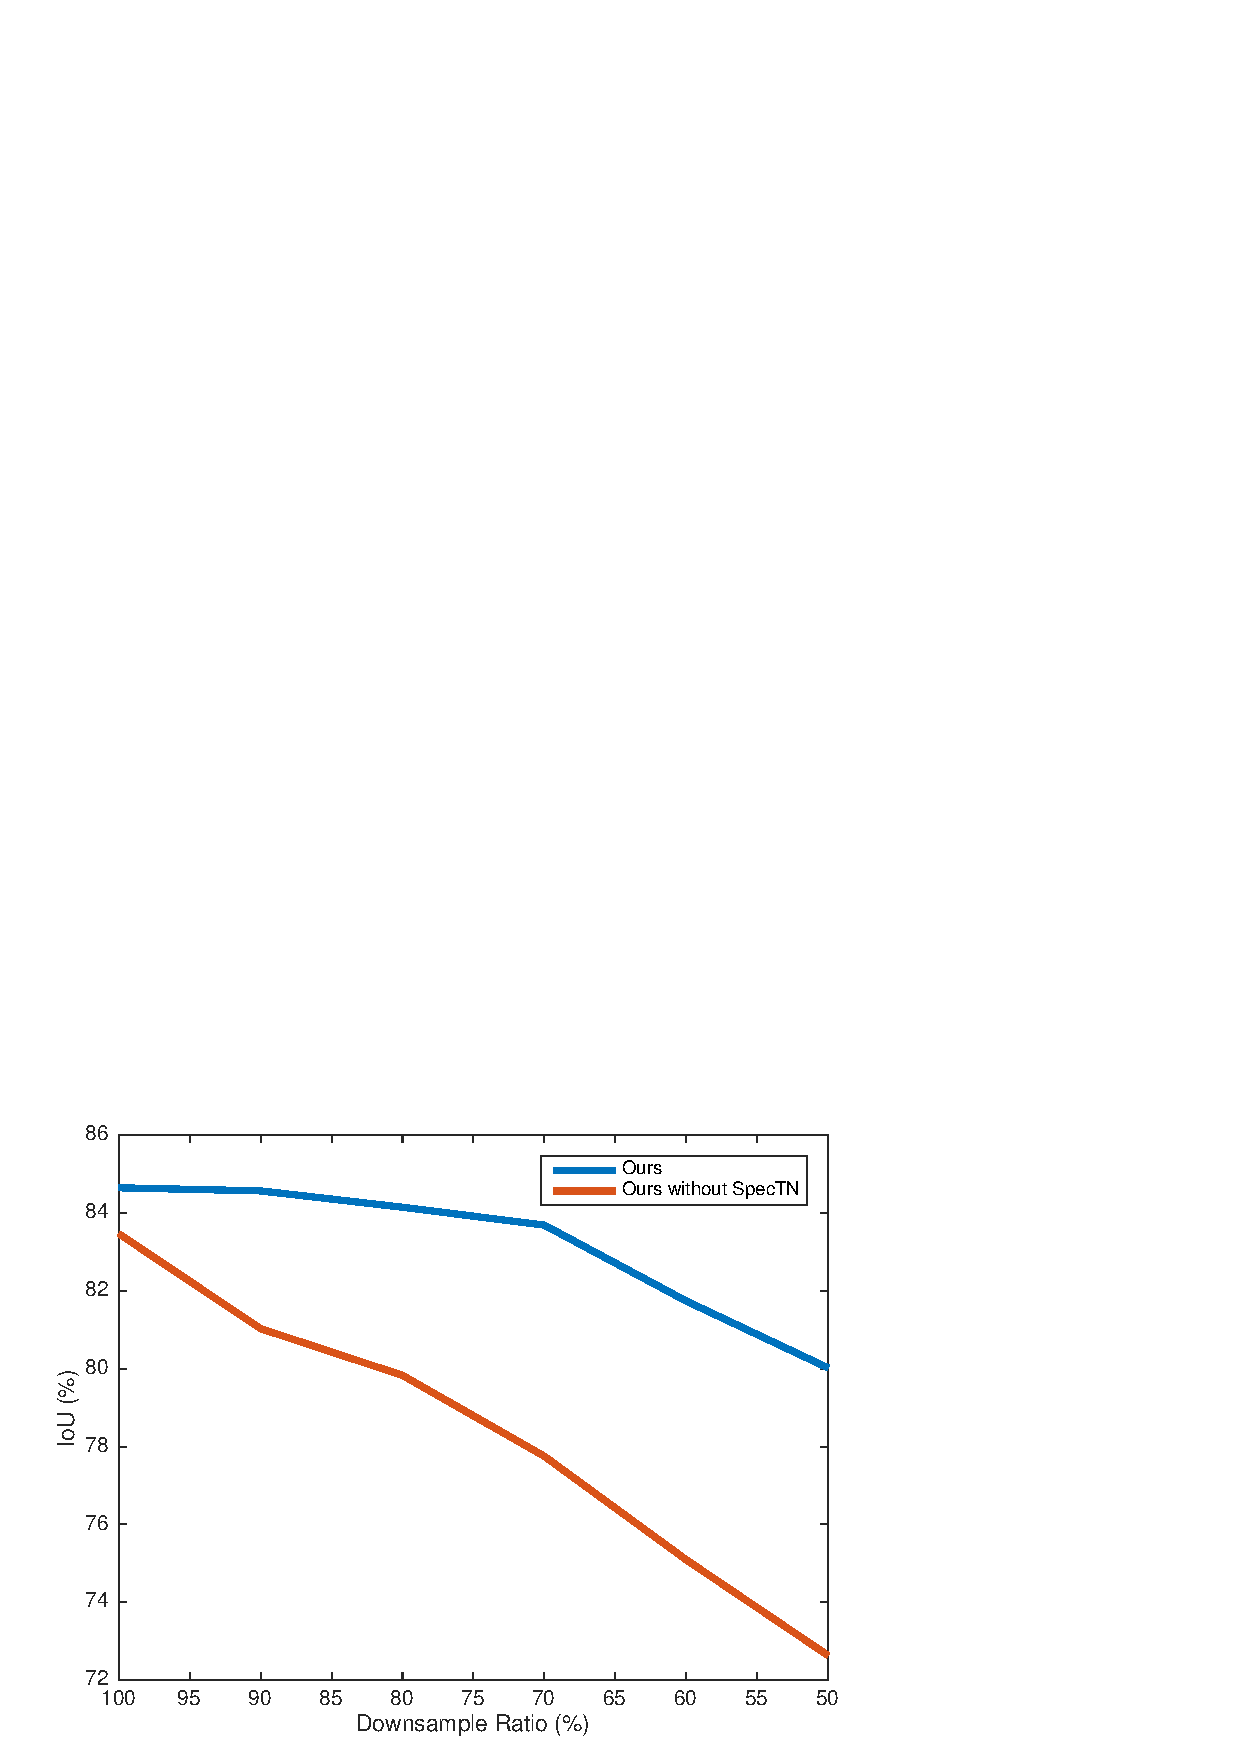
\includegraphics[width=0.8\linewidth]{./fig/downsample.pdf}
 \caption{We evaluate the robustness of our model to sampling density change. Test shapes are downsampled by different ratios and fed into our network. We compute the segmentation IoU for different downsample ratios and show it here. With SpecTN, our framework becomes more robust to sampling density change.}
 \label{fig:downsample}
\end{figure}

%\todo{Visualize joint basis}

\subsection{Qualitative Results and Error Analysis}
Figure~\ref{fig:erroranalysis} shows segmentation results generated from our network on two categories, Chair and Lamp. Representative good results are shown in the first block and  typical error patterns are summarized from the second to fourth blocks.

Most of our segmentation is very close to ground truth as is shown in the first block. We can accurately segment shapes with large geometric or topological variations like wide bench v.s. ordinary chair, pendant lamp v.s. table lamp. The lamp base on the first row and the lampshade on the second row are very similar regarding their local geometry; however, since our network is able to capture large scale context information, it could still differentiate the two and segment shapes correctly.

We observe several typical error patterns in our results. Most segmentation error occurs along part boundaries. %Our network sometimes generates fuzzy part boundaries, especially if the underlying part segments have a very smooth normal transition, as is shown in the second row of the second block. 
There are also cases where the semantic definition of parts has inherent ambiguities. %In these cases, our network may generate predictions slightly different from the ground truth but are still reasonable. 
We also observe a third type of error pattern, in which our prediction might miss a certain part completely, as is shown in the fourth block.

\begin{figure}
    \centering
    \includegraphics[width=\linewidth]{./fig/erroranalysis4.pdf}
    \caption{We visualize some segmentation results from our network prediction. The first block shows typical correct segmentations, notice the huge shape variation we can cover. The second to fourth blocks summarize different error patterns we observe in the results.}
    \label{fig:erroranalysis}
\end{figure}

\iffalse
\todo{
Compare different alternatives of our method
\begin{itemize}
    \item with multiple representatives instead of a single canonical space for spectral synchronization
    \item without join basis learning, visualize joint basis
    \item without dilated kernel, visualize dilated kernel
    \item different kernel choice: polynomial, cubic splines, exponential window, modulated exponential window
    \item different input vertex functions, extrinsic vertex functions help much since it's essentially a combination between extrinsic and intrinsic information for segmentation. intrinsic feature might not help much since the network is intrinsic and captures quite a lot intrinsic information already.
    \item network design, with/without skip link
\end{itemize}
}
\fi
\paragraph{3D Object Detection from RGB-D Data} Researchers have approached the 3D detection problem by taking various ways to represent RGB-D data.

\emph{Front view image based methods:} ~\cite{chen2016monocular, mousavian20163d, xiang2015data} take monocular RGB images and shape priors or occlusion patterns to infer 3D bounding boxes. ~\cite{li2016vehicle, deng2017amodal} represent depth data as 2D maps and apply CNNs to localize objects in 2D image. In comparison we represent depth as a point cloud and use advanced 3D deep networks (PointNets) that can exploit 3D geometry more effectively.

\emph{Bird's eye view based methods:} MV3D~\cite{cvpr17chen} projects LiDAR point cloud to bird's eye view and trains a region proposal network (RPN~\cite{ren2015faster}) for 3D bounding box proposal. However, the method lags behind in detecting small objects, such as pedestrians and cyclists and cannot easily adapt to scenes with multiple objects in vertical direction.
%Our method shares the idea with~\cite{cvpr17chen} in reducing 3D search cost by 2D search first. What differentiates our method from \cite{cvpr17chen} is that, \hao{???} instead of projecting point cloud to images costing loss in 3D geometry, we directly apply PointNet to point clouds that correspond to the 2D regions. % Besides, our method and MV3D can potentially be combined in the bird's eye setting. 3D proposals from our frustum-based PointNet and MV3D can be combined and our 3D network can also be used for bounding box estimation for point cloud in the bird's eye 2D region.

\emph{3D based methods:} ~\cite{wang2015voting, song2014sliding} train 3D object classifiers by SVMs on hand-designed geometry features extracted from point cloud and then localize objects using sliding-window search. \cite{engelcke2017vote3deep} extends ~\cite{wang2015voting} by replacing SVM with 3D CNN on voxelized 3D grids. \cite{ren2016three} designs new geometric features for 3D object detection in a point cloud. \cite{song2016deep, li20163d} convert a point cloud of the entire scene into a volumetric grid and use 3D volumetric CNN for object proposal and classification. Computation cost for those method is usually quite high due to the expensive cost of 3D convolutions and large 3D search space.
%In comparison, we use 2D region proposals from RGB images to reduce the search space from the entire 3D scenes into 3D frustums. Since the points cloud in the frustums have largely varying depth ranges and can be very sparse, it's not applicable to apply CNN on bird's eye view or apply 3D CNN in grids. Our frustum-based PointNet, on the other hand, suits well for this type of data and is able to accurately estimate 3D bounding box with good efficiency.
Recently, \cite{lahoud20172d} proposes a 2D-driven 3D object detection method that is similar to ours in spirit. However, they use hand-crafted features (based on histogram of point coordinates) with simple fully connected networks to regress 3D box location and pose, which is sub-optimal in both speed and performance. In contrast, we propose a more flexible and effective solution with deep 3D feature learning (PointNets).
%In addition we also get 3D instance segmentation as intermediate outputs. Evaluated on SUN-RGBD we show our method is \emph{8.9\%} better than theirs in mAP and \emph{34x} faster at the same time.


% \begin{enumerate}
%     \item ZOOX~\cite{mousavian20163d} image based
%     \item Vote3Deep~\cite{engelcke2017vote3deep} 3d cnn. Recent LIDAR-based methods place 3D windows in 3D voxel grids to score the point cloud
%     \item Voting for Voting~\cite{wang2015voting} Recent LIDAR-based methods place 3D windows in 3D voxel grids to score the point cloud. apply SVM classifers on 3D grids encoded with geometry features
%     \item MV3D~\cite{cvpr17chen}
%     \item VeloFCN~\cite{li2016vehicle} apply convolutional networks to the front view point map in a dense box prediction scheme
%     \item 3DOP~\cite{chen20153d} image based. reconstructs depth from stereo images and uses an energy minimization approach to generate 3D box proposals, which are fed to an R-CNN [10] pipeline for object recognition
%     \item Mono3D~\cite{chen2016monocular} image based. shares the same pipeline with 3DOP, it generates 3D proposals from monocular images.
%     \item 3DFCN~\cite{li20163d} 3d cnn.
%     \item 3DVP~\cite{xiang2015data} introduces 3D voxel patterns and employ a set of ACF detectors to do 2D detection and 3D pose estimation
%     \item Are Cars just 3D Box?~\cite{zeeshan2014cars} fit model to image patch
%     \item ~\cite{zia2013detailed} fit model to image patch
% \end{enumerate}
% \begin{enumerate}
%     \item SlidingShapes~\cite{song2014sliding} apply SVM classifers on 3D grids encoded with geometry features
%     \item DeepSlidingShapes~\cite{song2015sun} 3d cnn.
%     \item 2D-driven~\cite{lahoud20172d}
%     \item ~\cite{deng2017amodal} rgb-d images
%     \item COG feature~\cite{ren2016three}
%     \item Align 3D model in RGB-D~\cite{gupta2015aligning}
% \end{enumerate}

\paragraph{Deep Learning on Point Clouds}
Most existing works convert point clouds to images or volumetric forms before feature learning. \cite{wu20153d, maturana2015voxnet, qi2016volumetric} voxelize point clouds into volumetric grids and generalize image CNNs to 3D CNNs. ~\cite{li2016fpnn, riegler2016octnet, wang2017cnn, engelcke2017vote3deep} design more efficient 3D CNN or neural network architectures that exploit sparsity in point cloud.
However, these CNN based methods still require quantitization of point clouds with certain voxel resolution.
Recently, a few works~\cite{qi2017pointnet,qi2017pointnetplusplus} propose a novel type of network architectures (PointNets) that directly consumes raw point clouds without converting them to other formats. While PointNets have been applied to single object classification and semantic segmentation, our work explores how to extend the architecture for the purpose of 3D object detection.

%Conclusion!

%key,value for graph, duh duh duh
%]


We studied the problem of directly reading documents in order to answer questions,
concentrating our analysis on the gap between such direct methods and using
human-annotated or automatically constructed KBs.
We presented a new model, Key-Value Memory Networks, which helps bridge this gap,
outperforming several other methods across two datasets, \WikiMovies and {\sc WikiQA}.
However, some gap in performance still remains. \WikiMovies serves as an
 analysis tool to shed some light on the causes.
Future work should try to close this gap further.

Key-Value Memory Networks are versatile models for reading documents or KBs and answering
questions about them---allowing to encode prior knowledge about the task at hand
in the key and value memories. These models could be applied to storing and
reading memories
for other tasks as well, and future work should try them in other domains,
such as in a full dialog setting.
%dialog,
%for example dialgog




\subsubsection*{Acknowledgments}
This work was supported by the DARPA award D17AP00001, the Google focused award, and the Nvidia NVAIL award.

%
%Use unnumbered third level headings for the acknowledgments. All
%acknowledgments, including those to funding agencies, go at the end of the paper.

\clearpage

\bibliography{iclr2018_conference}
\bibliographystyle{iclr2018_conference}

\clearpage
\section{Positive Definiteness of~$K$}\label{sec:appendixA}
To show that the kernel~$K$ defined in~(\ref{eq:kernel}) is positive definite
(p.d.), we simply use elementary rules from the kernel literature described in
Sections 2.3.2 and 3.4.1 of~\cite{shawe2004}.  A linear combination of p.d. kernels with non-negative weights is also p.d. (see Proposition 3.22
of\cite{shawe2004}), and thus it is sufficient to show that for all $\z,\z'$
in~$\Omega$, the following kernel on $\Omega \to \HH$ is p.d.:
\begin{displaymath}
   (\varphi,\varphi') \mapsto \big\|\varphi(\z)\big\|_\HH  \normH{\varphi'(\z')} e^{-\frac{1}{2\sigma^2} \normH{\tildephi(\z)-\tildephi'(\z')}^2}.
\end{displaymath}
Specifically, it is also sufficient to
show that the following kernel on $\HH$ is p.d.:
\begin{displaymath}
   (\phi,\phi') \mapsto \big\|{\phi}\big\|_\HH  \normH{\phi'} e^{-\frac{1}{2\sigma^2} \normH{\frac{\phi}{\|\phi\|_\HH}-\frac{\phi'}{\|\phi'\|_\HH}}^2}.
\end{displaymath}
with the convention $\phi/\|\phi\|_\HH=0$ if~$\phi=0$.
This is a pointwise product of two kernels and is p.d. when each of the two
kernels is p.d. The first one is obviously p.d.: $(\phi,\phi') \mapsto
\|{\phi}\|_\HH  \normH{\phi'}$. The second one is a composition of the Gaussian
kernel---which is p.d.---, with feature maps $\phi/\|\phi\|_\HH$ of a
normalized linear kernel in~$\HH$.  This composition is p.d. according to
Proposition 3.22, item (v) of~\cite{shawe2004} since the normalization does
not remove the positive-definiteness property.

\section{List of Architectures Reported in the Experiments}\label{appendix:arch}
We present in details the architectures used in the paper in Table~\ref{table:arch}.
\begin{table}[hbtp]
   \centering
   \begin{tabular}{|*{9}{c|}}
      \hline
      Arch. & $N$ & $m_1$  & $p_1$  &  $\gamma_1$ & $m_2$ &  $p_2$ & $S$  &  $\sharp$ param\\
      \hline
      \hline
      \multicolumn{9}{|c|}{MNIST} \\
      \hline
      CKN-GM1 & 2 &  $1 \times 1$  &  12  & 2 &  $3 \times 3$ &  50 &  $4 \times 4$ & $5\,400$\\
      \hline
      CKN-GM2 & 2 &  $1 \times 1$  &  12  & 2 &  $3 \times 3$ &  400 &  $3 \times 3$& $43\,200$ \\
      \hline
      CKN-PM1 & 1 &  $5 \times 5$  &  200  & 2 &  - &  - &  $4 \times 4$  & $5\,000$ \\
      \hline
      CKN-PM2 & 2 &  $5 \times 5$  &  50  & 2 &  $2 \times 2$ &  200 &  $6 \times 6$ & $41\,250$ \\
      \hline
      \hline
      \multicolumn{9}{|c|}{CIFAR-10} \\
      \hline
      CKN-GM & 2 &  $1 \times 1$  &  12  & 2 &  $2 \times 2$ & 800 &  $4 \times 4$ & $38\,400$\\
      \hline
      CKN-PM & 2 &  $2 \times 2$  &  100  & 2 &  $2 \times 2$ &  800 &  $4 \times 4$ & $321\,200$\\
      \hline
      \hline
      \multicolumn{9}{|c|}{STL-10} \\
      \hline
      CKN-GM & 2 &  $1 \times 1$  &  12  & 2 &  $3 \times 3$ & 800 &  $4 \times 4$ & $86\,400$\\
      \hline
      CKN-PM & 2 &  $3 \times 3$  &  50  & 2 &  $3 \times 3$ &  800 &  $3 \times 3$ & $361\,350$\\
      \hline

   \end{tabular}
   \caption{List of architectures reported in the paper. $N$ is the number of layers; $p_1$ and~$p_2$ represent the number of filters are each layer; $m_1$ and~$m_2$ represent the size of the patches~$\NN_1$ and~$\NN_2$ that are of size~$m_1 \times m_1$ and~$m_2 \times m_2$ on their respective feature maps~$\zeta_1$ and~$\zeta_2$; $\gamma_1$ is the subsampling factor between layer 1 and layer 2; $S$ is the size of the output feature map, and the last column indicates the number of parameters that the network has to learn.}
   \label{table:arch}
\end{table}



\end{document}
